% chapters/02-entry-strategy.tex

\chapter{Building Your Entry Strategy}

\begin{importantbox}
This chapter provides a structured approach to developing your market entry strategy, with specific frameworks for different business types and regions. The tools and templates provided can be customized to your specific needs.
\end{importantbox}

\section{Choosing Your Market Entry Model}

\subsection{Entry Models Overview}
\begin{center}
\begin{tabular}{p{0.2\textwidth}|p{0.25\textwidth}|p{0.25\textwidth}|p{0.2\textwidth}}
    \textbf{Model} & \textbf{Advantages} & \textbf{Challenges} & \textbf{Best For} \\
    \hline
    Direct Entry & Full control & Higher resource needs & Established firms \\
    Partnership & Local knowledge & Shared control & New entrants \\
    Acquisition & Quick entry & Higher initial cost & Strategic buyers \\
    Representative & Lower risk & Limited control & Market testing \\
\end{tabular}
\end{center}

\subsection{Decision Framework}
\begin{figure}[h]
    \centering
    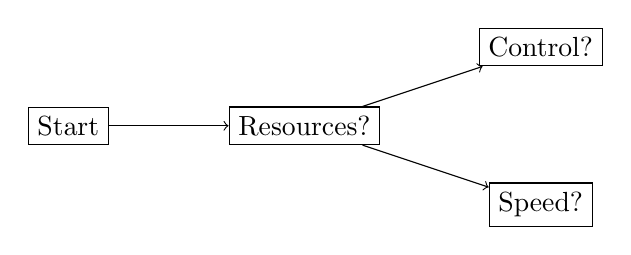
\begin{tikzpicture}
        % Decision tree for entry model selection
        \node[draw] (start) at (0,0) {Start};
        \node[draw] (resources) at (3,0) {Resources?};
        \node[draw] (control) at (6,1) {Control?};
        \node[draw] (speed) at (6,-1) {Speed?};

        \draw[->] (start) -- (resources);
        \draw[->] (resources) -- (control);
        \draw[->] (resources) -- (speed);
    \end{tikzpicture}
    \caption{Entry Model Decision Tree}
\end{figure}

\section{Legal Structures and Options}

\begin{warningbox}
Legal requirements can vary by sector and change over time. Always consult with qualified legal professionals for current requirements.
\end{warningbox}

\subsection{Common Legal Structures}
\begin{itemize}
    \item Private Limited Company
    \item Branch Office
    \item Representative Office
    \item Business Partnership
\end{itemize}

\section{Timeline and Resource Planning}

\begin{figure}[h]
    \centering
    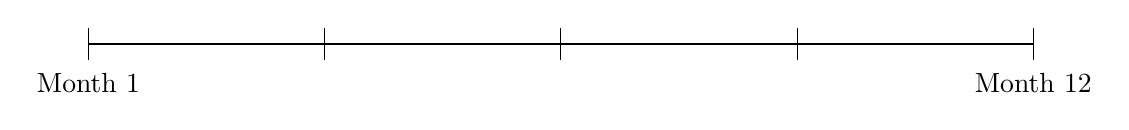
\begin{tikzpicture}
        % Timeline visualization
        \draw[thick] (0,0) -- (12,0);
        \foreach \x in {0,3,6,9,12}
            \draw (\x,0.2) -- (\x,-0.2);
        \node at (0,-0.5) {Month 1};
        \node at (12,-0.5) {Month 12};
    \end{tikzpicture}
    \caption{Typical Entry Timeline}
\end{figure}

\section{Regional Entry Pathways}

\begin{regionalbox}{United Kingdom}
\textbf{Financial Services Compliance Pathway}
\begin{itemize}
    \item Regulatory alignment requirements
    \item Capital adequacy standards
    \item Cross-border transaction frameworks
    \item UK-Nigeria financial corridors
\end{itemize}

\subsection{UK-Specific Process Flow}
\begin{enumerate}
    \item Initial compliance assessment
    \item Financial services licensing
    \item Local partnership development
    \item Operational setup
\end{enumerate}
\end{regionalbox}

\begin{regionalbox}{United States}
\textbf{Tech Startup Launch Framework}
\begin{itemize}
    \item IP protection strategy
    \item Tech infrastructure setup
    \item Digital service deployment
    \item Market testing approach
\end{itemize}

\subsection{US-Specific Process Flow}
\begin{enumerate}
    \item Market validation
    \item MVP development
    \item Beta testing
    \item Full launch
\end{enumerate}
\end{regionalbox}

\begin{regionalbox}{UAE}
\textbf{Trade License \& Import/Export Guide}
\begin{itemize}
    \item Trade license requirements
    \item Import/export documentation
    \item Logistics setup guide
    \item Trade finance options
\end{itemize}

\subsection{UAE-Specific Process Flow}
\begin{enumerate}
    \item Trade license acquisition
    \item Supply chain setup
    \item Partner network development
    \item Operations launch
\end{enumerate}
\end{regionalbox}

\begin{regionalbox}{Canada}
\textbf{Sector-Specific Entry Requirements}
\begin{itemize}
    \item Agricultural sector standards
    \item Environmental compliance
    \item Local partnership requirements
    \item Market access protocols
\end{itemize}

\subsection{Canada-Specific Process Flow}
\begin{enumerate}
    \item Sector compliance review
    \item Partnership development
    \item Operational planning
    \item Market entry execution
\end{enumerate}
\end{regionalbox}

\section{Risk Assessment Framework}

\begin{importantbox}
A comprehensive risk assessment should be conducted before finalizing your entry strategy.
\end{importantbox}

\begin{center}
\begin{tabular}{p{0.3\textwidth}|p{0.3\textwidth}|p{0.3\textwidth}}
    \textbf{Risk Category} & \textbf{Mitigation Strategies} & \textbf{Resources Required} \\
    \hline
    Regulatory & Compliance partners & Legal expertise \\
    Market & Phased entry & Market research \\
    Operational & Local partnerships & Operating procedures \\
    Financial & Risk management & Financial reserves \\
\end{tabular}
\end{center}

\begin{communitybox}
Access additional resources on the Africa Growth Circle:
\begin{itemize}
    \item Entry strategy templates
    \item Expert consultation sessions
    \item Peer review opportunities
    \item Regional success stories
\end{itemize}
Visit circle.counseal.com for more information.
\end{communitybox}

% End of chapter workshop
\begin{workshopbox}
\textbf{Chapter 2 Strategy Development Workshop}

1. Entry Model Selection
\begin{itemize}
    \item Preferred model: \_\_\_\_\_\_\_\_\_
    \item Key rationale: \_\_\_\_\_\_\_\_\_
    \item Resource requirements: \_\_\_\_\_\_\_\_\_
\end{itemize}

2. Timeline Development
\begin{itemize}
    \item Major milestones: \_\_\_\_\_\_\_\_\_
    \item Critical dependencies: \_\_\_\_\_\_\_\_\_
    \item Resource allocation: \_\_\_\_\_\_\_\_\_
\end{itemize}

3. Risk Assessment
\begin{itemize}
    \item Primary risks: \_\_\_\_\_\_\_\_\_
    \item Mitigation strategies: \_\_\_\_\_\_\_\_\_
    \item Contingency plans: \_\_\_\_\_\_\_\_\_
\end{itemize}

Download additional planning templates from the Africa Growth Circle platform.
\end{workshopbox}

\begin{importantbox}
In Chapter 3, we'll examine real-world success stories and learn from the experiences of entrepreneurs who have successfully entered the Nigerian market.
\end{importantbox}